\def\QRCODE{TB_image_TUT.IMG.machine_learning_pythonqrcode.png}
\def\QRPAGE{http://www.iptutorials.science/tree/master/TB_image/TUT.IMG.machine_learning/python}
\pcorrectionsection{Python correction}

The following imports may be considered.
\begin{python}
# image manipulation and features construction
import glob
from skimage import measure, io
import numpy as np
import matplotlib.pyplot as plt
# preprocessing data and normalization
from sklearn.preprocessing import StandardScaler
from sklearn.preprocessing.data import QuantileTransformer
# learning methods
from sklearn import svm
from sklearn.neural_network import MLPClassifier
from sklearn.model_selection import train_test_split
from sklearn.metrics import classification_report,confusion_matrix
# plot confusion matrix
import seaborn as sn
import pandas as pd
\end{python}

\subsection{Feature extraction}
We make a loop on the whole database to extract some features of each image. The 9 features used here are: area, convex area, eccentricity, equivalent diameter, extent, major axis length, minor axis length, perimeter and solidity. 

\begin{python}
# Definitions of the database, classes and images
rep = 'images_Kimia216/';
classes = ['bird','bone','brick','camel','car','children',
    'classic','elephant','face','fork','fountain',
    'glass','hammer','heart','key','misk','ray','turtle'];
nbClasses = len(classes);
nbImages = 12;
# The features are manually computed
properties = np.zeros((nbClasses*nbImages,9));
target = np.zeros(nbClasses * nbImages);
index=0;
for ind_c, c in enumerate(classes):
    filelist = glob.glob(rep+c+'*');
    for filename in filelist:
        I = io.imread(filename);
        prop = measure.regionprops(I);
        properties[index, 0] = prop[0].area;
        properties[index, 1] = prop[0].convex_area;
        properties[index, 2] = prop[0].eccentricity;
        properties[index, 3] = prop[0].equivalent_diameter;
        properties[index, 4] = prop[0].extent;
        properties[index, 5] = prop[0].major_axis_length;
        properties[index, 6] = prop[0].minor_axis_length;
        properties[index, 7] = prop[0].perimeter;
        properties[index, 8] = prop[0].solidity;
        target[index] = ind_c;
        
        index = index+1;
\end{python}

Note that in the same time, the target array (required in the following) is built within this loop. It represents the true classes of the objects.

\vspace*{-6pt}

\subsection{Classification}
We used a training set of $75\%$ of the database and $25\%$ for the test set. The scaler is used in order to rescale the data having different ranges and dimensions. Other scalers are proposed in \pinline{sklearn.preprocessing}.

\begin{python}
# percentage of the data used for splitting into train/test
percentTest = .25;
# MLP Classifier (Multi-Layer Perceptron)
# the data are first scaled
propertiesMLP = StandardScaler().fit_transform(properties);
prop_train, prop_test, target_train, target_test = train_test_split(propertiesMLP, target,test_size=percentTest, random_state=0);
\end{python}

\vspace*{-2pt}

The network is created with 1 hidden layers of 10 neurons. One could also use SVM instead of MLP (\pinline{classifier = svm.SVC(kernel='linear');}).

\begin{python}
# feedforward neural network
# max_iter should be extended max_iter=100000 for adam or sgd solvers
mlp = MLPClassifier(hidden_layer_sizes=(10,), solver='lbfgs');
target_pred = mlp.fit(prop_train, target_train).predict(prop_test)
print("Training set score: %f" % mlp.score(prop_train, target_train))
\end{python}

The training score should be around 1, according to the training dataset and the different parameters employed.
\begin{sh}
Training set score: 1.000000
\end{sh}

\vspace*{-8pt}

\subsection{Performance}
The confusion matrix gives an idea of the overall performance. The following function uses the modules \pinline{seaborn} and \pinline{pandas} to generate a \pinline{heatmap} that displays the confusion matrix.

\begin{python}
def plot_cm(cm, classes, normalize=False, cmap=plt.cm.Blues):
    """
    Plot confusion matrix
    cm: confusion matrix, as ouput by sklearn.metrics.confusion_matrix
    classes: labels to be used
    normalize: display number (False by default) or fraction (True)
    cmap: colormap
    returns: figure that can be used for pdf export
    """
    if normalize:
        cm = cm.astype('float') / cm.sum(axis=1)[:, np.newaxis] 
    fmt = '.1f' if normalize else 'd'
    df_cm = pd.DataFrame(cm, index = classes, columns = classes);
    
    fig = plt.figure();
    sn.set(font_scale=.8)
    sn.heatmap(df_cm, annot=True, cmap = cmap, fmt=fmt);
    plt.xlabel('Target label')
    plt.ylabel('True label')
    
    return fig;
\end{python}

The previous function is then used, and illustrated in Fig.\ref{fig:machine_learning:python:confusion}.
\begin{python}
cnf_matrix = confusion_matrix(target_test, target_pred);
fig=plot_cm(cnf_matrix, classes, normalize=True);
\end{python}

\pinline{sklearn.metrics.classification_report} can be used to display the performance.

\begin{sh}
             precision    recall  f1-score   support

       bird       0.75      1.00      0.86         3
       bone       1.00      1.00      1.00         5
      brick       1.00      1.00      1.00         1
      camel       1.00      1.00      1.00         3
        car       1.00      1.00      1.00         1
   children       1.00      1.00      1.00         2
    classic       1.00      1.00      1.00         5
   elephant       1.00      1.00      1.00         3
       face       1.00      1.00      1.00         4
       fork       1.00      1.00      1.00         2
   fountain       1.00      1.00      1.00         3
      glass       1.00      1.00      1.00         5
     hammer       1.00      0.75      0.86         4
      heart       1.00      1.00      1.00         2
        key       1.00      1.00      1.00         3
       misk       1.00      1.00      1.00         3
        ray       1.00      1.00      1.00         4
     turtle       1.00      1.00      1.00         1

avg / total       0.99      0.98      0.98        54
\end{sh}

\begin{figure}[H]
\centering
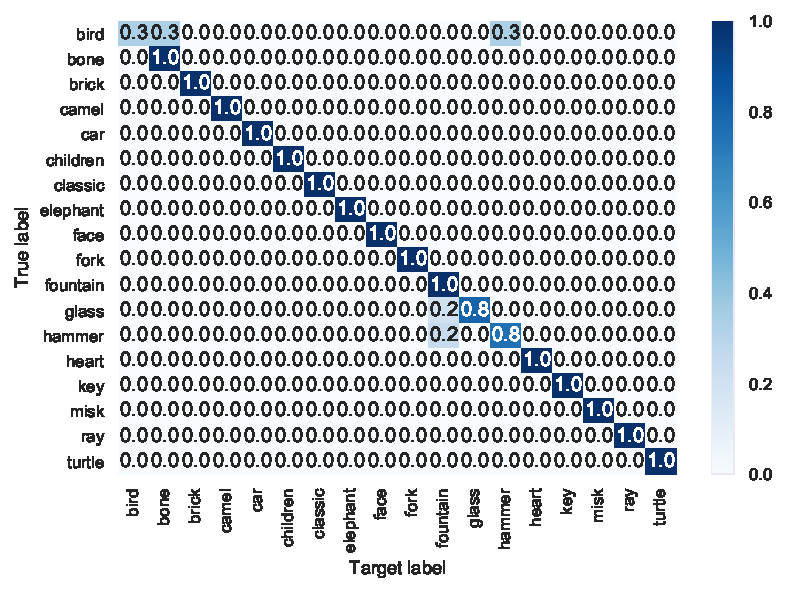
\includegraphics[width=.8\linewidth]{confusion_norm_mlp.pdf}
\caption{Normalized confusion matrix of the classification result.}
 \label{fig:machine_learning:python:confusion}
\end{figure}
